\documentclass{article}
\usepackage{graphics} 
\usepackage{hyperref}

\author{Kevin Zollicoffer}
\title{Predictive Modeling\\Lesson 4a\\\emph{Linear Regression and Regression Trees}}
\date{10/06/2013}

\usepackage{Sweave}
\begin{document}
\maketitle
%\tableofcontents
\Sconcordance{concordance:Assignment4a.tex:Assignment4a.Rnw:%
1 8 1 1 0 11 1 1 2 1 0 1 2 4 1 1 2 19 0 1 2 3 1 1 2 1 0 4 1 3 0 1 2 2 1 %
1 2 1 0 1 1 33 0 2 2 117 0 1 2 6 0 1 2 1 1 5 0 1 2 1 1 6 0 1 2 4 1 1 10 %
9 0 1 2 2 1 1 2 23 0 1 1 27 0 1 3 2 1 2 2 4 1 1 2 24 0 1 1 27 0 1 3 1 1 %
2 2 4 1 1 2 24 0 1 1 27 0 1 3 1 1 2 2 7 1 1 3 8 0 1 2 8 1}


\section*{Introduction}
The RStudio project files and accompanying artifacts, including the tex file that created this PDF, are publicly available on GitHub
\\
\url{https://github.com/zollie/PASS-PredictiveModeling-LinearRegressionAndRegressionTrees}

\section*{Data Setup}
I took the Excel spreadsheet and saved it as a CSV for easy import into R
\begin{Schunk}
\begin{Sinput}
> bh <- read.csv("~/R/PASS/PredictiveModeling/LinearRegressionAndRegressionTrees/BostonHousing.csv")
> bh$X <- NULL
> bh$X.1 <- NULL
> bh$X.2 <- NULL
> bh$X.3 <- NULL
> bh$X.4 <- NULL
> head(bh)
\end{Sinput}
\begin{Soutput}
     CRIM ZN INDUS CHAS   NOX    RM  AGE    DIS RAD TAX PTRATIO      B LSTAT
1 0.00632 18  2.31    0 0.538 6.575 65.2 4.0900   1 296    15.3 396.90  4.98
2 0.02731  0  7.07    0 0.469 6.421 78.9 4.9671   2 242    17.8 396.90  9.14
3 0.02729  0  7.07    0 0.469 7.185 61.1 4.9671   2 242    17.8 392.83  4.03
4 0.03237  0  2.18    0 0.458 6.998 45.8 6.0622   3 222    18.7 394.63  2.94
5 0.06905  0  2.18    0 0.458 7.147 54.2 6.0622   3 222    18.7 396.90  5.33
6 0.02985  0  2.18    0 0.458 6.430 58.7 6.0622   3 222    18.7 394.12  5.21
  MEDV
1 24.0
2 21.6
3 34.7
4 33.4
5 36.2
6 28.7
\end{Soutput}
\end{Schunk}


\section*{Partitioning}
Next, the data is paritioned into 60\% Train and 40\% Test sets. I set the RNG seed for reproducibility
\begin{Schunk}
\begin{Sinput}
> set.seed(21275)
> n <- nrow(bh)
> a <- sort(sample(1:n, floor(n*.6)))
> bh.train <- bh[a,]
> bh.test <- bh[-a,]
\end{Sinput}
\end{Schunk}

\section*{Linear Regression}
A Linear Regression model is fit to the train data. Then the model is used to make predictions using the test data while calculating the standard error for the Root Standard Mean Error
\begin{Schunk}
\begin{Sinput}
> mlr <- lm(MEDV ~ ., data=bh.test)
> summary(mlr)
\end{Sinput}
\begin{Soutput}
Call:
lm(formula = MEDV ~ ., data = bh.test)

Residuals:
     Min       1Q   Median       3Q      Max 
-10.4756  -2.8634  -0.4371   1.6646  22.1601 

Coefficients:
              Estimate Std. Error t value Pr(>|t|)    
(Intercept)  27.888067   7.848307   3.553  0.00048 ***
CRIM         -0.106956   0.072117  -1.483  0.13971    
ZN            0.049067   0.021667   2.265  0.02467 *  
INDUS        -0.022680   0.103597  -0.219  0.82695    
CHAS          4.518344   1.451186   3.114  0.00214 ** 
NOX         -13.912872   5.965888  -2.332  0.02075 *  
RM            4.156809   0.634901   6.547 5.38e-10 ***
AGE          -0.003258   0.022165  -0.147  0.88328    
DIS          -1.545232   0.331761  -4.658 6.02e-06 ***
RAD           0.250664   0.100892   2.484  0.01384 *  
TAX          -0.012236   0.005920  -2.067  0.04010 *  
PTRATIO      -0.603644   0.219315  -2.752  0.00649 ** 
B             0.009321   0.004173   2.234  0.02668 *  
LSTAT        -0.594316   0.081152  -7.324 6.78e-12 ***
---
Signif. codes:  0 ‘***’ 0.001 ‘**’ 0.01 ‘*’ 0.05 ‘.’ 0.1 ‘ ’ 1

Residual standard error: 4.735 on 189 degrees of freedom
Multiple R-squared:  0.7511,	Adjusted R-squared:  0.734 
F-statistic: 43.87 on 13 and 189 DF,  p-value: < 2.2e-16
\end{Soutput}
\begin{Sinput}
> mlr.pred <- predict(mlr, newdata=bh.test, se.fit=TRUE)
> head(mlr.pred)
\end{Sinput}
\begin{Soutput}
$fit
        4         6         7        10        14        18        21        22 
29.714160 25.957478 21.777154 17.219889 20.764395 17.644027 12.636732 18.441022 
       28        31        35        39        42        45        46        47 
15.237105 11.492917 14.056023 23.444027 28.588449 22.792016 21.834889 19.925409 
       49        55        58        60        63        67        70        71 
 7.017180 15.961282 32.702779 21.315283 24.472685 24.706993 20.821867 25.633714 
       72        76        79        82        84        87        88        89 
21.753825 23.886646 20.856452 27.503854 25.484312 22.159385 26.228971 31.443007 
       94        96        97        98        99       100       102       109 
29.237393 29.210982 24.781005 36.967139 36.412615 33.125572 27.055993 23.611240 
      112       114       115       116       118       120       121       129 
26.671856 20.117934 25.157003 19.902148 23.577127 20.415539 21.658533 19.696195 
      130       132       133       136       137       138       142       143 
14.337696 20.322249 21.063828 17.859595 16.371248 20.181758  2.956121 14.788836 
      146       148       150       153       154       156       160       161 
10.572343  6.529505 13.612512 21.228043 16.504114 21.414881 25.632117 33.647218 
      167       169       171       172       174       180       181       185 
36.988119 25.110348 20.859110 22.757070 28.922533 33.839084 35.645994 22.400581 
      186       187       188       191       194       196       199       200 
24.759640 37.131160 33.042259 30.436935 32.076026 40.932312 33.562971 30.584081 
      201       208       209       213       219       223       224       225 
31.203131 17.172166 25.039173 24.161332 25.420127 33.913340 29.746350 39.208190 
      228       229       230       231       239       240       243       244 
32.670880 36.316493 31.694445 23.992847 28.169229 28.051000 23.286563 27.178362 
      246       248       249       250       251       254       255       259 
12.438906 19.652636 21.329564 24.550954 24.690852 31.122316 23.563944 36.053773 
      262       263       267       271       272       273       276       282 
36.862921 41.065728 30.243691 22.277313 27.858715 29.059152 34.432398 33.911158 
      283       285       286       287       292       294       295       296 
42.048737 31.316309 26.682996 19.979341 35.689282 24.797868 23.147904 27.707513 
      297       301       302       306       307       310       314       317 
26.411145 29.987932 28.219071 31.280262 36.488668 23.781892 25.948645 17.118145 
      320       321       322       328       330       331       332       334 
21.382657 25.699561 25.679832 19.618868 24.293379 21.340947 19.349591 23.325918 
      335       340       343       344       347       348       350       352 
22.662304 22.123640 21.925966 28.091464 14.560947 25.581120 23.389614 20.868084 
      357       361       364       366       368       370       373       376 
21.281707 23.230933 21.983244 13.771885  9.625910 34.933418 27.839945 25.475565 
      378       383       386       389       390       393       394       395 
19.661775 12.346955  6.414429  4.659947 13.260512  8.493454 19.941827 17.471469 
      399       401       402       403       405       409       410       411 
 4.966028 10.725885 17.217942 17.679711  6.095118 12.077657 19.108860 14.812751 
      414       417       421       425       427       431       432       435 
10.458996 12.502894 19.470933 13.634894 15.602735 17.346477 17.874907 15.727103 
      436       438       440       446       452       454       455       456 
12.819864  7.888171 12.228805 11.331696 19.127613 22.521070 14.959344 15.499756 
      457       462       465       470       472       473       478       479 
12.098358 20.026672 20.059396 17.810058 22.161287 21.869056  9.939112 18.378290 
      481       482       484       485       487       490       491       493 
22.887545 26.868539 20.404695 18.826205 18.863572  7.369337  2.297218 16.046951 
      498       500       501 
19.334566 18.556162 20.751059 

$se.fit
        4         6         7        10        14        18        21        22 
0.9317122 0.9286232 0.9094579 1.3495501 0.9596900 0.8568180 1.0481473 0.9126928 
       28        31        35        39        42        45        46        47 
0.9851723 1.0701011 1.1519041 0.9932167 1.1800970 0.7483313 0.8446413 0.9018019 
       49        55        58        60        63        67        70        71 
1.7794641 1.5922848 1.5564002 0.9109190 1.1569029 1.2860336 0.7725690 1.1564554 
       72        76        79        82        84        87        88        89 
1.0128518 0.8096550 0.8126226 0.7673139 0.6196457 0.7741901 0.7510598 0.9635369 
       94        96        97        98        99       100       102       109 
1.3273137 0.8869292 0.9095414 1.1938209 1.2027777 0.9482638 0.9636533 1.0114876 
      112       114       115       116       118       120       121       129 
0.7861166 0.8913017 0.8514661 0.8658377 0.8390837 0.8693890 2.0296093 1.2028232 
      130       132       133       136       137       138       142       143 
1.1014328 1.2365316 1.2677682 1.1732646 1.1102194 1.2100763 1.5857398 1.8387206 
      146       148       150       153       154       156       160       161 
1.6867581 1.6959211 1.4868280 1.8779506 1.5288533 2.0221573 1.7158873 1.7186939 
      167       169       171       172       174       180       181       185 
1.5950180 1.2528310 1.2415745 1.2755666 0.9358624 0.9258309 1.1054596 1.1862111 
      186       187       188       191       194       196       199       200 
0.9103022 1.0603503 1.2290780 1.0142139 1.0315543 1.3364976 1.3680617 1.4427962 
      201       208       209       213       219       223       224       225 
1.4590041 0.7923440 1.5322894 1.5936021 1.6335361 1.5200233 0.7754441 1.1506324 
      228       229       230       231       239       240       243       244 
0.8031847 1.3200924 1.1129999 0.7363773 0.7528767 0.6163152 0.8381933 0.9002992 
      246       248       249       250       251       254       255       259 
1.2682497 1.3727987 0.9264054 0.9588302 0.9070551 1.7184301 1.2578433 1.3560648 
      262       263       267       271       272       273       276       282 
1.3009348 1.4853447 1.3177693 0.8587378 1.0828205 0.7609909 0.9198071 0.8714906 
      283       285       286       287       292       294       295       296 
1.6319925 1.2964835 0.8933280 1.3238859 1.6415385 1.2856638 1.1934003 1.2735060 
      297       301       302       306       307       310       314       317 
1.2809873 1.1569262 0.7263730 1.1260704 1.1987212 0.6510009 0.7153293 0.6890953 
      320       321       322       328       330       331       332       334 
0.5460082 0.6508959 0.6595567 0.7389261 1.5305962 1.4041473 0.8229418 1.1700935 
      335       340       343       344       347       348       350       352 
1.1470084 0.9609671 1.6945314 0.8575222 1.3107864 1.2464621 1.3070139 1.5901144 
      357       361       364       366       368       370       373       376 
1.5813572 1.3553720 1.5945469 2.3036478 1.9795235 1.7539784 1.6002766 1.3011771 
      378       383       386       389       390       393       394       395 
1.0419006 0.9365723 1.2273389 1.1725238 0.9367140 1.0314995 0.8582648 0.8736632 
      399       401       402       403       405       409       410       411 
2.1448516 1.3834186 0.9098533 0.8568119 2.2633278 1.1588585 1.0855765 3.1845183 
      414       417       421       425       427       431       432       435 
1.5001348 1.5206493 0.8170834 1.5613504 1.4655408 1.2358307 1.3200201 1.0956961 
      436       438       440       446       452       454       455       456 
1.1792701 1.4020738 0.9782476 1.3342367 0.9675572 1.2111130 1.4224180 1.3642674 
      457       462       465       470       472       473       478       479 
1.4867771 1.0244533 0.9380025 1.0017059 1.1757307 0.9986555 0.9628734 0.8341819 
      481       482       484       485       487       490       491       493 
1.0452997 1.1415572 1.2419500 1.1851493 0.9518138 1.8225458 1.9199579 1.8731892 
      498       500       501 
0.7372024 0.8533092 0.7142648 

$df
[1] 189

$residual.scale
[1] 4.734828
\end{Soutput}
\begin{Sinput}
> summary(mlr.pred$se.fit)
\end{Sinput}
\begin{Soutput}
   Min. 1st Qu.  Median    Mean 3rd Qu.    Max. 
 0.5460  0.9097  1.1560  1.1870  1.3660  3.1850 
\end{Soutput}
\begin{Sinput}
> se <-mean(mlr.pred$se.fit)
> se
\end{Sinput}
\begin{Soutput}
[1] 1.186619
\end{Soutput}
\begin{Sinput}
> rse <- sqrt(se)
> rse
\end{Sinput}
\begin{Soutput}
[1] 1.08932
\end{Soutput}
\end{Schunk}

\section*{Regression Trees}

First a function is created to build Regresstion Trees with varying paremeters. Next, this function is used to build Regression Trees.

\begin{Schunk}
\begin{Sinput}
> f <- function(minspl, minbuck) {
+   require(rpart)
+   require(rpart.plot)
+   
+   rtree <- rpart(MEDV ~., data=bh.train, method="anova", minsplit=minspl, minbucket=minbuck)
+   
+   # pruned with min xerror
+   rtree.pruned <- prune(rtree, rtree$cptable[which.min(rtree$cptable[,"xerror"]),"CP"])  
+ }
> rtree.A <- f(3, 1)
> rtree.B <- f(10, 3)
> rtree.C <- f(30, 1)
> printcp(rtree.A)
\end{Sinput}
\begin{Soutput}
Regression tree:
rpart(formula = MEDV ~ ., data = bh.train, method = "anova", 
    minsplit = minspl, minbucket = minbuck)

Variables actually used in tree construction:
[1] CRIM  DIS   LSTAT RM   

Root node error: 25689/303 = 84.781

n= 303 

        CP nsplit rel error  xerror     xstd
1 0.479933      0   1.00000 1.01169 0.109182
2 0.170368      1   0.52007 0.61426 0.073748
3 0.050214      2   0.34970 0.43368 0.059815
4 0.044850      3   0.29949 0.42787 0.063684
5 0.036171      4   0.25464 0.39895 0.063174
6 0.029695      5   0.21846 0.35276 0.062554
7 0.023446      6   0.18877 0.34427 0.062468
\end{Soutput}
\begin{Sinput}
> rsq.rpart(rtree.A)
\end{Sinput}
\begin{Soutput}
Regression tree:
rpart(formula = MEDV ~ ., data = bh.train, method = "anova", 
    minsplit = minspl, minbucket = minbuck)

Variables actually used in tree construction:
[1] CRIM  DIS   LSTAT RM   

Root node error: 25689/303 = 84.781

n= 303 

        CP nsplit rel error  xerror     xstd
1 0.479933      0   1.00000 1.01169 0.109182
2 0.170368      1   0.52007 0.61426 0.073748
3 0.050214      2   0.34970 0.43368 0.059815
4 0.044850      3   0.29949 0.42787 0.063684
5 0.036171      4   0.25464 0.39895 0.063174
6 0.029695      5   0.21846 0.35276 0.062554
7 0.023446      6   0.18877 0.34427 0.062468
\end{Soutput}
\begin{Sinput}
> #plotcp(rtree.A)
\end{Sinput}
\end{Schunk}

\begin{figure}
\begin{center}
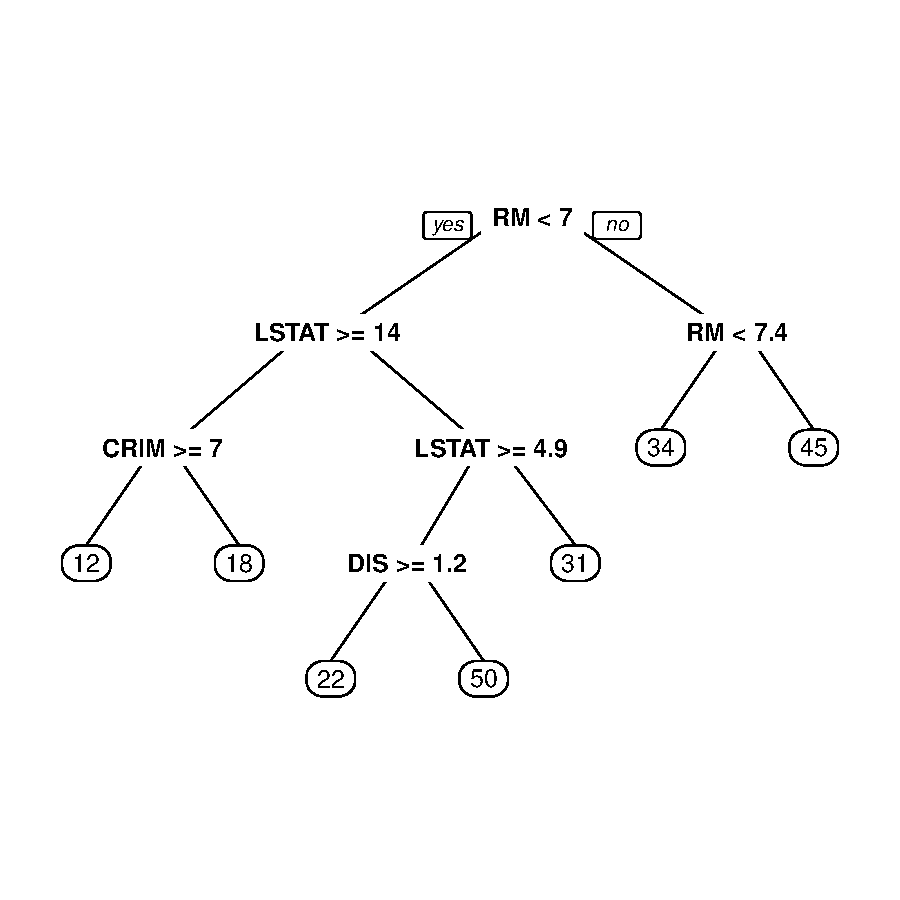
\includegraphics{Assignment4a-005}
\end{center}
\caption{rtree.A}
\label{rtree:A}
\end{figure}

\begin{Schunk}
\begin{Sinput}
> printcp(rtree.B)
\end{Sinput}
\begin{Soutput}
Regression tree:
rpart(formula = MEDV ~ ., data = bh.train, method = "anova", 
    minsplit = minspl, minbucket = minbuck)

Variables actually used in tree construction:
[1] CRIM  LSTAT RM   

Root node error: 25689/303 = 84.781

n= 303 

        CP nsplit rel error  xerror     xstd
1 0.479933      0   1.00000 1.00559 0.108379
2 0.170368      1   0.52007 0.59992 0.072855
3 0.050214      2   0.34970 0.42661 0.059573
4 0.044850      3   0.29949 0.42154 0.062043
5 0.036171      4   0.25464 0.38942 0.062886
6 0.019601      5   0.21846 0.34383 0.061656
7 0.016124      6   0.19886 0.32647 0.061155
\end{Soutput}
\begin{Sinput}
> rsq.rpart(rtree.B)
\end{Sinput}
\begin{Soutput}
Regression tree:
rpart(formula = MEDV ~ ., data = bh.train, method = "anova", 
    minsplit = minspl, minbucket = minbuck)

Variables actually used in tree construction:
[1] CRIM  LSTAT RM   

Root node error: 25689/303 = 84.781

n= 303 

        CP nsplit rel error  xerror     xstd
1 0.479933      0   1.00000 1.00559 0.108379
2 0.170368      1   0.52007 0.59992 0.072855
3 0.050214      2   0.34970 0.42661 0.059573
4 0.044850      3   0.29949 0.42154 0.062043
5 0.036171      4   0.25464 0.38942 0.062886
6 0.019601      5   0.21846 0.34383 0.061656
7 0.016124      6   0.19886 0.32647 0.061155
\end{Soutput}
\begin{Sinput}
> #plotcp(rtree.B)
\end{Sinput}
\end{Schunk}
\begin{figure}
\begin{center}
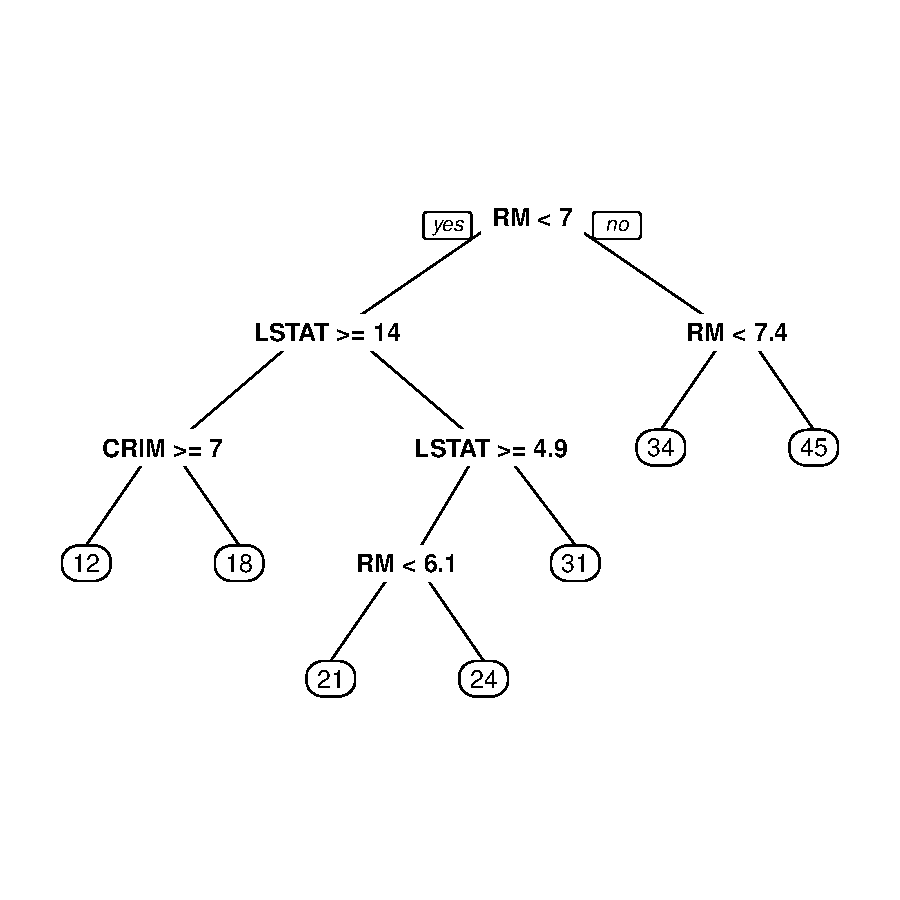
\includegraphics{Assignment4a-007}
\end{center}
\caption{rtree.B}
\label{rtree:B}
\end{figure}

\begin{Schunk}
\begin{Sinput}
> printcp(rtree.C)
\end{Sinput}
\begin{Soutput}
Regression tree:
rpart(formula = MEDV ~ ., data = bh.train, method = "anova", 
    minsplit = minspl, minbucket = minbuck)

Variables actually used in tree construction:
[1] CRIM  DIS   LSTAT RM   

Root node error: 25689/303 = 84.781

n= 303 

        CP nsplit rel error  xerror     xstd
1 0.479933      0   1.00000 1.00489 0.108849
2 0.170368      1   0.52007 0.58880 0.072471
3 0.050214      2   0.34970 0.45249 0.062622
4 0.044850      3   0.29949 0.42235 0.061164
5 0.036171      4   0.25464 0.39002 0.062550
6 0.029695      5   0.21846 0.36871 0.062673
7 0.015811      6   0.18877 0.35734 0.062362
\end{Soutput}
\begin{Sinput}
> rsq.rpart(rtree.C)
\end{Sinput}
\begin{Soutput}
Regression tree:
rpart(formula = MEDV ~ ., data = bh.train, method = "anova", 
    minsplit = minspl, minbucket = minbuck)

Variables actually used in tree construction:
[1] CRIM  DIS   LSTAT RM   

Root node error: 25689/303 = 84.781

n= 303 

        CP nsplit rel error  xerror     xstd
1 0.479933      0   1.00000 1.00489 0.108849
2 0.170368      1   0.52007 0.58880 0.072471
3 0.050214      2   0.34970 0.45249 0.062622
4 0.044850      3   0.29949 0.42235 0.061164
5 0.036171      4   0.25464 0.39002 0.062550
6 0.029695      5   0.21846 0.36871 0.062673
7 0.015811      6   0.18877 0.35734 0.062362
\end{Soutput}
\begin{Sinput}
> #plotcp(rtree.C)
\end{Sinput}
\end{Schunk}
\begin{figure}
\begin{center}
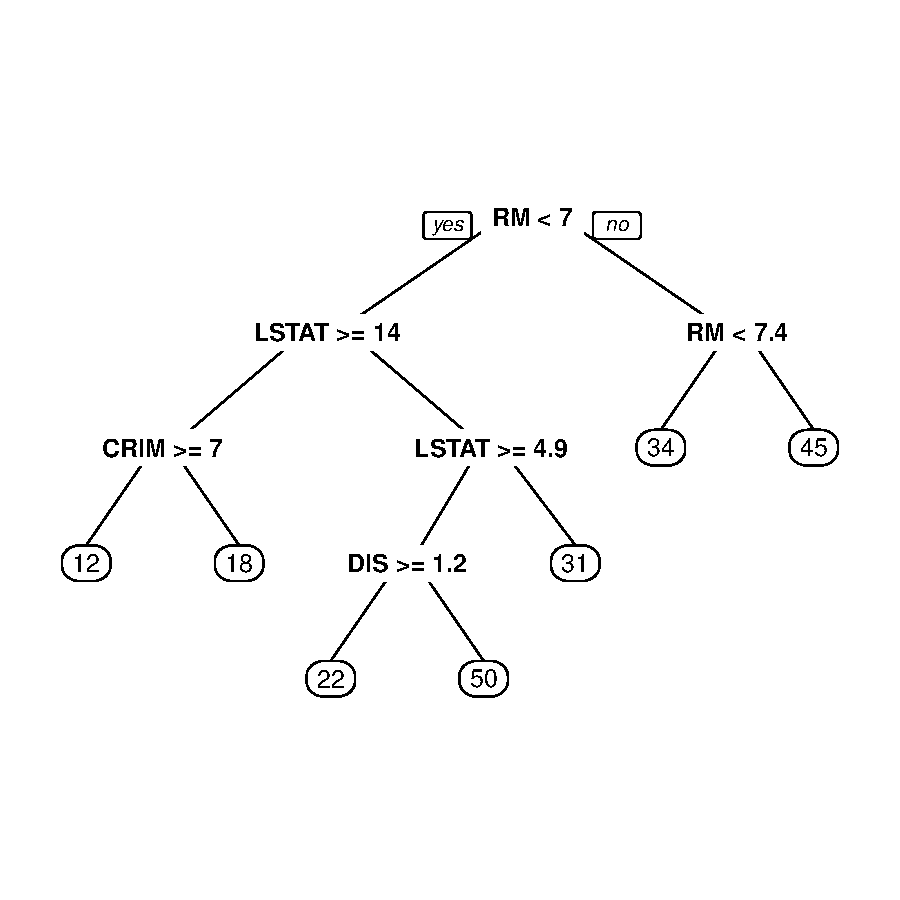
\includegraphics{Assignment4a-009}
\end{center}
\caption{rtree.C}
\label{rtree:C}
\end{figure}

\section*{Lesson 4a Question and Answer}
\subsection*1\emph{Report the root mean squared error on the validation data}

\begin{Schunk}
\begin{Sinput}
> # root standard mean error from above
> rse
\end{Sinput}
\begin{Soutput}
[1] 1.08932
\end{Soutput}
\end{Schunk}

\subsection*2\emph{Use the regression tree procedure in XLMiner to develop several models to predict the median value of houses in census tracts. Try multiple combinations of the tuning parameters}
\newline
\newline
\noindent
See Above. 


\end{document}
